%add subsections like this
\subsection{Introduction}
Octave can solve Linear Programming problems using the glpk function. That is, Octave can solve

\newenvironment{centerverbatim}{%
  \par
  \centering
  \varwidth{\linewidth}%
  \verbatim
}{%
  \endverbatim
  \endvarwidth
  \par
}

\begin{verbatim}
min C'*x
\end{verbatim}

subject to the linear constraints
\begin{equation}
A*x = b \;\;\;\; \text{where} \; x \geq 0
\end{equation}

the \textbf{glpk} function also supports variations of this problem.

\subsection{Syntax}
\begin{verbatim}
    : [xopt, fmin, errnum, extra] = glpk (c, A, b, lb, ub, ctype, vartype, sense, param)
\end{verbatim}

Given 3 Parameters, \textbf{gplk} solves the following standard form linear programming problem:

\begin{equation}
\begin{aligned}
\min & \; c^T x \\
\text{subject to} & \; A x = b \\
x \geq 0
\end{aligned}
\end{equation}

but it can also solve the following variations of this problem:

% center code
\begin{centerverbatim}
[min|max] c'*x
\end{centerverbatim}

subject to the linear constraints
\begin{centerverbatim}
    A*x [ "=" | "<=" | ">=" ] b
    x >= LB
    x <= UB
\end{centerverbatim}

\subsection{Parameters and Flags}
 
%inject .pdf
\setboolean{@twoside}{false}
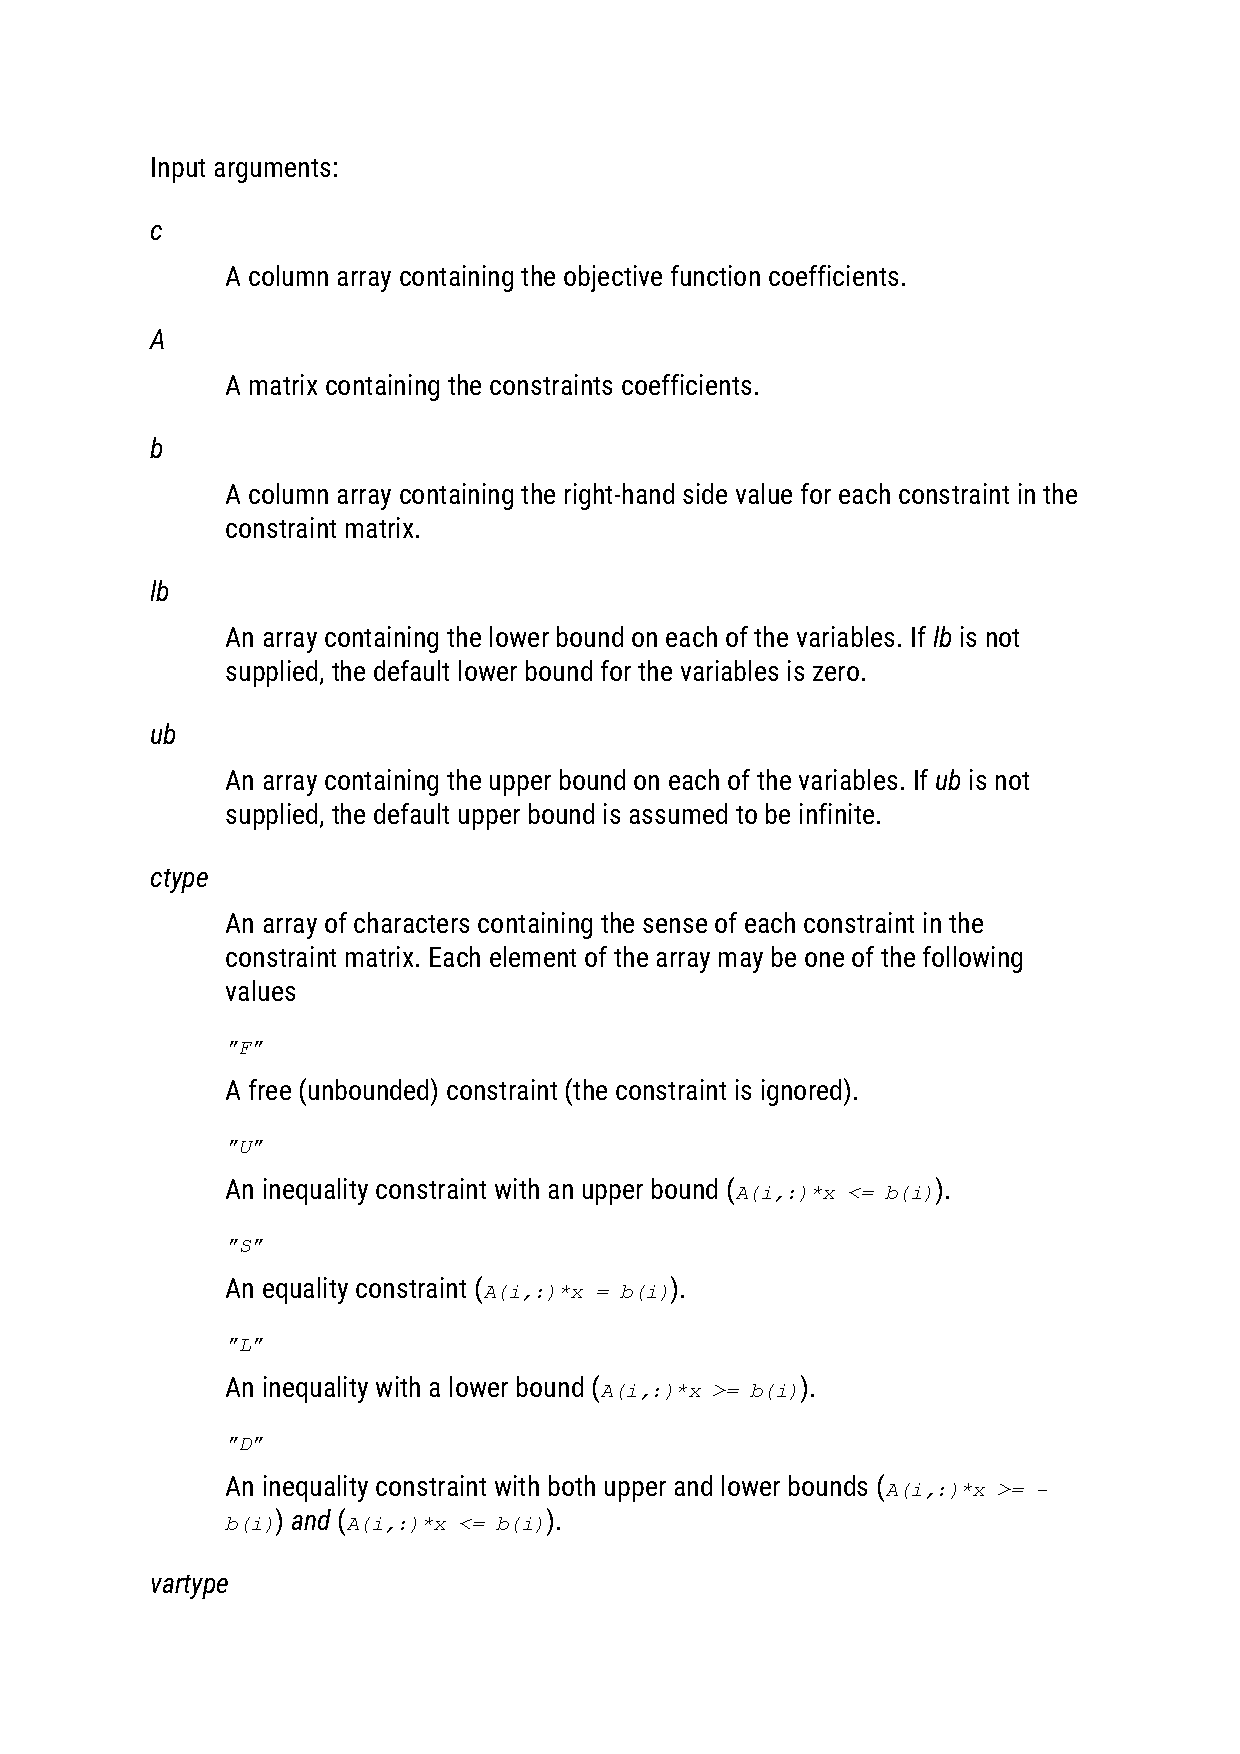
\includepdf[pages=-]{chapters/manual.pdf}